\chapter{EM algorithm}
\label{chap:EM-algorithm}


\section{Jensen's inequality}

\subsection{Convex function}
\begin{definition}
A real valued function $f : X \rightarrow R$ defined on a convex set $X$ in a vector space is called \textbf{convex function} if, for any two points $\vec{x}_1$ and  $\vec{x}_2$  in $X$ and any $\lambda \in [0,1]$,
\begin{equation}
f(\lambda \vec{x}_1 + (1 - \lambda)\vec{x}_2) \leq \lambda f(\vec{x}_1) + (1 - \lambda)f(\vec{x}_2)
\end{equation}

The function $f$ is said to be \textbf{strictly convex} if
\begin{equation}
f(\lambda \vec{x}_1 + (1 - \lambda)\vec{x}_2) < \lambda f(\vec{x}_1) + (1 - \lambda)f(\vec{x}_2)
\end{equation}
\end{definition}

\begin{definition}
A function $f$ is said to be (strictly) \textbf{concave} if $-f$ is (strictly) convex.
\end{definition}

\begin{theorem}
If $f(x)$ is twice differentiable on $[a, b]$ and $f''(x) \geq 0$ on $[a, b]$ then $f(x)$ is convex on $[a, b]$.
\end{theorem}

\begin{proposition}
$\log(x)$ is strictly convex on $(0, \infty)$.
\end{proposition}


\subsection{Jensen's inequality}
\begin{theorem}
Let $f$ be a convex function defined on a convex set $X$ . If $\vec{x}_1, \vec{x}_2, \cdots , \vec{x}_n \in X$ and $\lambda_1, \lambda_2, \cdots , \lambda_n \geq 0$ with $\sum\limits_{i=1}^n \lambda_i=1$,
\begin{equation}
f\left(\sum\limits_{i=1}^n \lambda_i\vec{x}_i\right) \leq \sum\limits_{i=1}^n {\lambda_i f(\vec{x}_i)}
\end{equation}
\end{theorem}

\begin{proposition}
\begin{equation}
\log\left(\sum\limits_{i=1}^n \lambda_i\vec{x}_i\right) \geq \sum\limits_{i=1}^n {\lambda_i \log(\vec{x}_i)}
\end{equation}
\end{proposition}


\section{EM algorithm}
The EM algorithm is an efficient iterative procedure to compute the Maximum Likelihood (ML) estimate in the presence of missing or hidden data. 

Each iteration of the EM algorithm consists of two processes: The E-step, and the M-step. In the expectation, or E-step, the missing data are estimated given the observed data and current estimate of the model parameters. This is achieved using the conditional expectation, explaining the choice of terminology. In the M-step, the likelihood function is maximized under the assumption that the missing data are known. The estimate of the missing data from the E-step are used in lieu of the actual missing data.

\begin{algorithm}[htbp]
    \SetKwInOut{Input}{input}\SetKwInOut{Output}{output}
    \Input{observed data $\mathcal{X}=\{\vec{x}^{(1)},\vec{x}^{(2)},\cdots, \vec{x}^{(n)}$\},joint distribution $P(\mathcal{X},\vec{z}|\vec{\theta})$}
	\Output{model's parameters $\vec{\theta}$}

	// 1. identify hidden variables $\vec{z}$, write out the log likelihood function $\ell(\mathcal{X},\vec{z}|\vec{\theta})$ \\
	$\vec{\theta}^{(0)}$ = ... // initialize \\
	
	\While{(!convergency)} {
	    // 2. E-step: plug in $P(\mathcal{X},\vec{z}|\vec{\theta})$, derive the formula of $Q(\vec{\theta}, \vec{\theta}^{(i)})$ \\
	    $Q(\vec{\theta}, \vec{\theta}^{(i)})=\mathbb{E}_{\vec{z}|\mathcal{X},\vec{\theta}^{(i)}}\left[\log P(\mathcal{X},\vec{z}|\vec{\theta})\right]$ \\
	    // 3. M-step: find \vec{\theta} that maximizes the value of $Q(\vec{\theta}, \vec{\theta}^{(i)})$ \\
		$\vec{\theta}^{(i+1)}=\arg\max\limits_{\vec{\theta}} Q(\vec{\theta}, \vec{\theta}^{(i)})$ \\
	}
	
\caption{EM algorithm}
\end{algorithm}

\section{Derivation of the EM algorithm}
The log likelihood function is given by 
\begin{eqnarray}
\ell(\vec{\theta}) &=& \log{P(\mathcal{X}|\vec{\theta})} \text{ ,where } \log{P(\mathcal{X}|\vec{\theta})}=\sum\limits_{i=1}^{n} \log{{P(\vec{x}^{(i)}|\vec{\theta})}}\nonumber \\
                &=& \log{{\sum\limits_{\vec{z}} P(\mathcal{X},\vec{z}|\vec{\theta})}} \nonumber \\
				&=& \log{{\sum\limits_{\vec{z}} P(\mathcal{X}|\vec{z},\vec{\theta})P(\vec{z}|\vec{\theta})}} \nonumber \\
\ell(\vec{\theta})-\ell(\vec{\theta}^{(i)}) &=& \log\left[\sum\limits_{\vec{z}} P(\mathcal{X}|\vec{z},\vec{\theta})P(\vec{z}|\vec{\theta})\right] - \log{P(\mathcal{X}|\vec{\theta}^{(i)})} \nonumber \\
                &=& \log\left[\sum\limits_{\vec{z}} P(\mathcal{X}|\vec{z},\vec{\theta})P(\vec{z}|\vec{\theta})\dfrac{P(\vec{z}|\mathcal{X},\theta^{(i)})}{P(\vec{z}|\mathcal{X},\theta^{(i)})}\right] - \log{P(\mathcal{X}|\vec{\theta}^{(i)})} \nonumber \\
				&=& \log\left[\sum\limits_{\vec{z}} P(\vec{z}|\mathcal{X},\theta^{(i)})\dfrac{P(\mathcal{X}|\vec{z},\vec{\theta})P(\vec{z}|\vec{\theta})}{P(\vec{z}|\mathcal{X},\theta^{(i)})}\right] - \log{P(\mathcal{X}|\vec{\theta}^{(i)})} \nonumber \\
				&\geq& \sum\limits_{\vec{z}} P(\vec{z}|\mathcal{X},\theta^{(i)})\log\left[\dfrac{P(\mathcal{X}|\vec{z},\vec{\theta})P(\vec{z}|\vec{\theta})}{P(\vec{z}|\mathcal{X},\theta^{(i)})}\right] - \log{P(\mathcal{X}|\vec{\theta}^{(i)})} \nonumber \\
				&=& \sum\limits_{\vec{z}} P(\vec{z}|\mathcal{X},\theta^{(i)})\log\left[\dfrac{P(\mathcal{X}|\vec{z},\vec{\theta})P(\vec{z}|\vec{\theta})}{P(\vec{z}|\mathcal{X},\theta^{(i)})P(\mathcal{X}|\vec{\theta}^{(i)})}\right] \nonumber \\
				&\triangleq& B(\vec{\theta},\vec{\theta}^{(i)}) \nonumber \\
\Rightarrow \nonumber
\end{eqnarray}

\begin{eqnarray}
\vec{\theta}^{(i+1)} &=& \arg\max\limits_{\vec{\theta}}{\left[ \ell(\vec{\theta}^{(i)})+B(\vec{\theta},\vec{\theta}^{(i)})\right]} \nonumber \\
                &=& \arg\max\limits_{\vec{\theta}}{\left\{ \ell(\vec{\theta}^{(i)})+\sum\limits_{\vec{z}} P(\vec{z}|\mathcal{X},\theta^{(i)})\log\left[\dfrac{P(\mathcal{X}|\vec{z},\vec{\theta})P(\vec{z}|\vec{\theta})}{P(\vec{z}|\mathcal{X},\theta^{(i)})P(\mathcal{X}|\vec{\theta}^{(i)})}\right]\right\}} \nonumber \\
				&& \text{Now drop terms which are constant w.r.t. } \vec{\theta} \nonumber \\
				&=& \arg\max\limits_{\vec{\theta}}{\left\{\sum\limits_{\vec{z}} P(\vec{z}|\mathcal{X},\theta^{(i)})\log\left[P(\mathcal{X}|\vec{z},\vec{\theta})P(\vec{z}|\vec{\theta})\right]\right\}} \nonumber \\
				&=& \arg\max\limits_{\vec{\theta}}{\left\{\sum\limits_{\vec{z}} P(\vec{z}|\mathcal{X},\theta^{(i)})\log\left[P(\mathcal{X},\vec{z}|\vec{\theta})\right]\right\}} \nonumber \\
				&=& \arg\max\limits_{\vec{\theta}}{\left\{\mathbb{E}_{\vec{z}|\mathcal{X},\theta^{(i)}}\log\left[P(\mathcal{X},\vec{z}|\vec{\theta})\right]\right\}} \\
				&\triangleq& \arg\max\limits_{\vec{\theta}}{Q(\vec{\theta}, \vec{\theta}^{(i)})}
\end{eqnarray}

\begin{figure}[hbtp]
\centering
    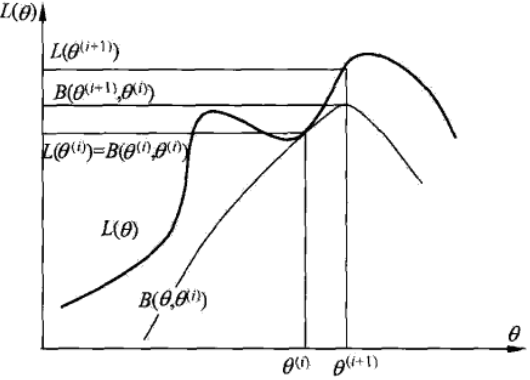
\includegraphics[scale=.50]{EM-algorithm.png}
\caption{Graphical interpretation of a single iteration of the EM algorithm: The function $B(\vec{\theta},\vec{\theta}^{(i)})$ is bounded above by the log likelihood function $\ell(\vec{\theta})$. The functions are equal at $\vec{\theta} = \vec{\theta}^{(i)}$. The EM algorithm chooses $\vec{\theta}^{(i)}$ as the value of $\vec{\theta}$ for which $B(\vec{\theta},\vec{\theta}^{(i)})$ is a maximum. Since $\ell(\vec{\theta}) \geq B(\vec{\theta},\vec{\theta}^{(i)})$ increasing $B(\vec{\theta},\vec{\theta}^{(i)})$ ensures that the value of the log likelihood function $\ell(\vec{\theta})$ is increased at each step.}
\label{fig:EM-algorithm} 
\end{figure}


\section{Examples}

\subsection{Gaussian mixture model}
\begin{definition}
In Gaussian mixture model(GMM) model, each base distribution in the mixture is a multivariate Gaussian with mean $\mu_k$ and covariance matrix $\sigma_k$. Thus the model has the form
\begin{equation}
P(x_i|\vec{\theta})=\sum\limits_{k=1}^K{\pi_k\phi(x_i|\mu_k,\sigma_k)}
\end{equation}
\end{definition}

Figure ~\ref{fig:GMM} shows a mixture of 3 Gaussians in 2D. Each mixture component is represented by a different set of eliptical contours. Given a sufficiently large number of mixture components, a GMM can be used to approximate any density defined on $\mathbb{R}^D$.

\begin{figure}[hbtp]
\centering
    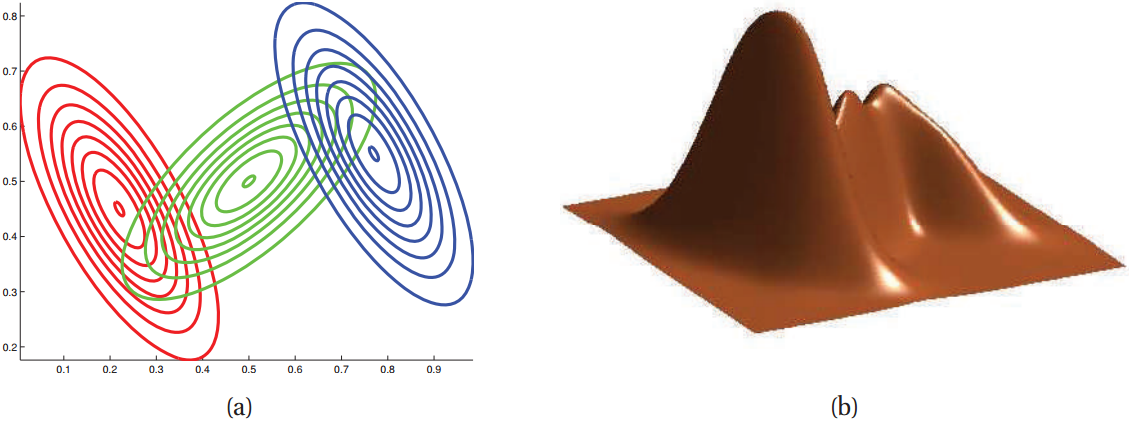
\includegraphics[scale=.50]{GMM.png}
\caption{A mixture of 3 Gaussians in 2d. (a) We show the contours of constant probability for eachcomponent in the mixture. (b) A surface plot of the overall density.}
\label{fig:GMM} 
\end{figure}


\subsubsection{Identify hidden variable, write out the log likelihood function}
Denote the hidden variable as $\gamma_{jk}$, which's meanining is:
\begin{equation}\nonumber
\gamma_{jk}=\begin{cases}
1, & \text{the j-th sample comes from the k-th model}\\
0, & \text{otherwise} \\
\end{cases}
\end{equation}

Given observed sample $x_j$ and hidden variable $\gamma_{jk}$, the complete sample is $(x_j,\gamma_{j1},\gamma_{j1},\cdots,\gamma_{jk})$.

Then the log likelihood function can be written as follows:
\begin{eqnarray}
P(\mathcal{X},\gamma|\vec{\theta}) &=& \prod\limits_{j=1}^N P(x_j,\gamma_{j1},\gamma_{j1},\cdots,\gamma_{jk}|\vec{\theta})\nonumber \\
       &=& \prod\limits_{j=1}^N\left\{\prod\limits_{k=1}^K\left[\pi_k\phi(x_i|\mu_k,\sigma_k)\right]^{\gamma_{jk}}\right\} \nonumber \\
	   &=& \prod\limits_{k=1}^K\left\{\prod\limits_{j=1}^N\left[\pi_k\phi(x_i|\mu_k,\sigma_k)\right]^{\gamma_{jk}}\right\} \nonumber \\
	   &=& \prod\limits_{k=1}^K\left\{\pi_k^{n_k}\prod\limits_{j=1}^N\left[\phi(x_i|\mu_k,\sigma_k)\right]^{\gamma_{jk}}\right\} \nonumber \\
	   &=& \prod\limits_{k=1}^K\left\{\pi_k^{n_k}\prod\limits_{j=1}^N\left[\dfrac{1}{\sqrt{2\pi}\Sigma_k}\exp{\left(-\dfrac{\left(x_j-\mu_k\right)^2}{2\sigma_k^2}\right)}\right]^{\gamma_{jk}}\right\} \nonumber \\
	   && \text{where } n_k=\sum\limits_{j=1}^N{\gamma_{jk}}, \sum\limits_{k=1}^K{n_k}=N. \nonumber \\
\Rightarrow \nonumber \\
\log{P(\mathcal{X},\gamma|\vec{\theta})} &=& \sum\limits_{k=1}^K\left\{n_k\log\pi_k+\sum\limits_{j=1}^N{\gamma_{jk}\left[\log(\dfrac{1}{\sqrt{2\pi}}-\log\sigma_k-\dfrac{\left(x_j-\mu_k\right)^2}{2\sigma_k^2})\right]}\right\}
\end{eqnarray}


\subsubsection{E-step: derive the formula of $Q(\vec{\theta}, \vec{\theta}^{(i)})$}
\begin{eqnarray}
Q(\vec{\theta}, \vec{\theta}^{(i)}) &=& \mathbb{E}_{\vec{z}|\mathcal{X},\theta^{(i)}}\log\left[P(\mathcal{X},\vec{z}|\vec{\theta})\right] \nonumber \\
    &=& \mathbb{E}_{\vec{\gamma}|\mathcal{X},\theta^{(i)}}\left\{\sum\limits_{k=1}^K\left\{n_k\log\pi_k+\sum\limits_{j=1}^N{\gamma_{jk}\left[\log(\dfrac{1}{\sqrt{2\pi}}-\log\sigma_k-\dfrac{\left(x_j-\mu_k\right)^2}{2\sigma_k^2})\right]}\right\}\right\} \nonumber \\
	&=& \sum\limits_{k=1}^K\left\{\left(\sum\limits_{j=1}^N{E\gamma_{jk}}\right)\log\pi_k+\sum\limits_{j=1}^N{E\gamma_{jk}\left[\log(\dfrac{1}{\sqrt{2\pi}}-\log\sigma_k-\dfrac{\left(x_j-\mu_k\right)^2}{2\sigma_k^2})\right]}\right\} \nonumber \\
	&& \text{denote } E\gamma_{jk} \text{ as } \hat{\gamma}_{jk} \nonumber \\
	&=& \sum\limits_{k=1}^K\left\{\left(\sum\limits_{j=1}^N{\hat{\gamma}_{jk}}\right)\log\pi_k+\sum\limits_{j=1}^N{\hat{\gamma}_{jk}\left[\log(\dfrac{1}{\sqrt{2\pi}}-\log\sigma_k-\dfrac{\left(x_j-\mu_k\right)^2}{2\sigma_k^2})\right]}\right\} \label{eqn:Q-function} \label{eqn:Q-function}
\end{eqnarray}

\begin{eqnarray}
\hat{\gamma}_{jk} &=& E\gamma_{jk} = E(\gamma_{jk}|x_j,\vec{\theta})=E(\gamma_{jk}=1|x_j,\vec{\theta}) \nonumber \\
	&=& \dfrac{P(\gamma_{jk}=1, x_j|\vec{\theta})}{\sum\limits_{k=1}^K{P(\gamma_{jk}=1, x_j|\vec{\theta})}} \nonumber \\
	&=& \dfrac{P(x_j|\gamma_{jk}=1, \vec{\theta})P(\gamma_{jk}=1, \vec{\theta})}{\sum\limits_{k=1}^K{P(x_j|\gamma_{jk}=1, \vec{\theta})P(\gamma_{jk}=1, \vec{\theta})}} \nonumber \\
	&=& \dfrac{\phi(x_i|\mu_k,\sigma_k)\pi_k}{\sum\limits_{k=1}^K{\phi(x_i|\mu_k,\sigma_k)\pi_k}} \nonumber \\
	&=& \dfrac{\pi_k\phi(x_i|\mu_k,\sigma_k)}{\sum\limits_{k=1}^K{\pi_k\phi(x_i|\mu_k,\sigma_k)}} \nonumber
\end{eqnarray}
Use this formula to update $\hat{\gamma}_{jk}$.

\subsubsection{M-step: find \vec{\theta} that maximizes the value of $Q(\vec{\theta}, \vec{\theta}^{(i)})$}
Take partial derivatives of Eqn.\eqref{eqn:Q-function} with respect to $\mu_k$, $\sigma_k^2$ and let them equal to 0, we can get $\mu_k$, $\sigma_k^2$.
\begin{eqnarray}
\dfrac{\partial}{\partial \mu_k}Q(\vec{\theta}, \vec{\theta}^{(i)}) &=& \sum\limits_{j=1}^N{\hat{\gamma}_{jk}\left[-\dfrac{1}{2\sigma_k^2} \cdot 2\left(x_j-\mu_k\right) \cdot (-1)\right]} = 0 \nonumber \\
\sum\limits_{j=1}^N{\hat{\gamma}_{jk}\left[\left(x_j-\mu_k\right)\right]} &=& 0 \nonumber \\
\hat{\mu}_k &=& \dfrac{\sum\limits_{j=1}^N{\hat{\gamma}_{jk}x_j}}{\hat{\gamma}_{jk}}
\end{eqnarray}

\begin{eqnarray}
\dfrac{\partial}{\partial \sigma_k^2}Q(\vec{\theta}, \vec{\theta}^{(i)}) &=& \sum\limits_{j=1}^N{\hat{\gamma}_{jk}\left[-\dfrac{1}{2\sigma_k^2}+\dfrac{1}{2\sigma_k^4}\left(x_j-\mu_k\right)^2\right]} = 0 \nonumber \\
\sum\limits_{j=1}^N{\hat{\gamma}_{jk}\left[-\sigma_k^2+\left(x_j-\mu_k\right)^2\right]} &=& 0 \nonumber \\
\hat{\sigma}_k^2 &=& \dfrac{\sum\limits_{j=1}^N{\hat{\gamma}_{jk}\left(x_j-\mu_k\right)^2}}{\hat{\gamma}_{jk}}
\end{eqnarray}

Grouping together only the terms that depend on $\pi_k$, we find that we need to maximize $\sum\limits_{k=1}^K{\left(\sum\limits_{j=1}^N{\hat{\gamma}_{jk}}\right)\log\pi_k}$. However, there is an additional constraint $\sum\limits_{k=1}^K{\pi_k}=1$, since they represent the probabilities $\vec{\pi}_k=P(x^{(i)}=k|\vec{\pi})$. To deal with the constraint we construct the Lagrangian
\begin{equation}
\mathcal{L}(\vec{\pi})=\sum\limits_{k=1}^K{\left(\sum\limits_{j=1}^N{\hat{\gamma}_{jk}}\right)\log\pi_k}+\beta\left(\sum\limits_{k=1}^K{\pi_k}-1\right) \nonumber
\end{equation}

where $\beta$ is the Lagrange multiplier. Taking derivatives, we find
\begin{equation}
\hat{\vec{\pi}}_k=\dfrac{\sum\limits_{k=1}^K{\hat{\gamma}_{jk}}}{N}
\end{equation}


\subsubsection{EM algorithm for GMM}

\begin{algorithm}[htbp]
    \SetAlgoNoLine
    \SetKwInOut{Input}{input}\SetKwInOut{Output}{output}
    \Input{observed data $\mathcal{X}=\{\vec{x}^{(1)},\vec{x}^{(2)},\cdots, \vec{x}^{(n)}$\},GMM}
	\Output{GMM's parameters $\vec{\pi},\vec{\mu},\vec{\sigma}$}

	// 1. initialize \\
	$\vec{\pi}^{(0)}$ = ... \\
	$\vec{\mu}^{(0)}$ = ...  \\
	$\vec{\sigma}^{(0)}$ = ...  \\
	
	\While{(!convergency)} {
	    // 2. E-step \\
	    $\hat{\gamma}_{jk}=\dfrac{\pi_k\phi(x_i|\mu_k,\sigma_k)}{\sum\limits_{k=1}^K{\pi_k\phi(x_i|\mu_k,\sigma_k)}}$ \\
	    // 3. M-step \\
		$\hat{\mu}_k = \dfrac{\sum\limits_{j=1}^N{\hat{\gamma}_{jk}x_j}}{\hat{\gamma}_{jk}}$ \\
		$\hat{\sigma}_k^2 = \dfrac{\sum\limits_{j=1}^N{\hat{\gamma}_{jk}\left(x_j-\mu_k\right)^2}}{\hat{\gamma}_{jk}}$ \\
		$\hat{\vec{\pi}}_k=\dfrac{\sum\limits_{k=1}^K{\hat{\gamma}_{jk}}}{N}$ \\
	}
	
\caption{EM algorithm for GMM}
\end{algorithm}


\section{Generalization of EM Algorithm}
EM algorithm can be interpreted as F function's maximization-maximization algorithm, based on this interpretation there are many variations and generalization, e.g., generalized EM Algorithm(GEM).


\subsection{F function's maximization-maximization algorithm}
\begin{definition}
Given the probability distribution of the hidden variable $Z$ is $\tilde{P}(Z)$, define \textbf{F function} as the following:
\begin{equation}
F(\tilde{P},\vec{\theta})=\mathbb{E}_{\tilde{P}}\left[\log{P(X,Z|\theta)}\right]+H(\tilde{P})
\end{equation}
Where $H(\tilde{P})=-\mathbb{E}_{\tilde{P}}\log\tilde{P}(Z)$, which is $\tilde{P}(Z)$'s entropy. Usually we assume that $P(X,Z|\theta)$ is continuous w.r.t. $\vec{\theta}$, therefore $F(\tilde{P},\vec{\theta})$ is continuous w.r.t. $\tilde{P}$ and $\vec{\theta}$.
\end{definition}

\begin{lemma}
\label{lemma:F-function}
For a fixed $\vec{\theta}$, there is only one distribution $\tilde{P}_{\theta}$ which maximizes $F(\tilde{P},\vec{\theta})$
\begin{equation}
\tilde{P}_{\theta}(Z)=P(Z|X, \vec{\theta})
\end{equation}
and $\tilde{P}_{\theta}$ is continuous w.r.t. $\vec{\theta}$.
\end{lemma}

\begin{proof}
Given a fixed $\vec{\theta}$, we can get $\tilde{P}_{\theta}$ which maximizes $F(\tilde{P},\vec{\theta})$. we construct the Lagrangian
\begin{equation}
\mathcal{L}(\tilde{P}, \vec{\theta})=\mathbb{E}_{\tilde{P}}\left[\log{P(X,Z|\theta)}\right]-\mathbb{E}_{\tilde{P}}\log\tilde{P}_{\theta}(Z)+\lambda\left[1-\sum\limits_Z{\tilde{P}(Z)}\right]
\end{equation}

Take partial derivative with respect to $\tilde{P}_{\theta}(Z)$ then we get
\begin{equation}
\dfrac{\partial \mathcal{L}}{\partial{\tilde{P}_{\theta}(Z)}}=\log{P(X,Z|\theta)}-\log\tilde{P}_{\theta}(Z)-1-\lambda  \nonumber
\end{equation}

Let it equal to 0, we can get
\begin{equation}
\lambda=\log{P(X,Z|\theta)}-\log\tilde{P}_{\theta}(Z)-1 \nonumber
\end{equation}

Then we can derive that $\tilde{P}_{\theta}(Z)$ is proportional to $P(X,Z|\theta)$
\begin{eqnarray}
\dfrac{P(X,Z|\theta)}{\tilde{P}_{\theta}(Z)} &=& e^{1+\lambda} \nonumber \\
\Rightarrow \tilde{P}_{\theta}(Z) &=& \dfrac{P(X,Z|\vec{\theta})}{e^{1+\lambda}} \nonumber \\
\sum\limits_Z{\tilde{P}_{\theta}(Z)}=1 & \Rightarrow & \sum\limits_Z{\dfrac{P(X,Z|\vec{\theta})}{e^{1+\lambda}}}=1 \Rightarrow P(X|\vec{\theta})=e^{1+\lambda} \nonumber \\
\tilde{P}_{\theta}(Z) &=& \dfrac{P(X,Z|\vec{\theta})}{e^{1+\lambda}} = \dfrac{P(X,Z|\vec{\theta})}{P(X|\vec{\theta})}=P(Z|X, \vec{\theta}) \nonumber
\end{eqnarray}
\end{proof}

\begin{lemma}
If $\tilde{P}_{\theta}(Z)=P(Z|X, \vec{\theta})$, then
\begin{equation}
F(\tilde{P},\vec{\theta})=\log P(X|\vec{\theta})
\end{equation}
\end{lemma}

\begin{theorem}
One iteration of EM algorithm can be implemented as F function's maximization-maximization.

Assume $\vec{\theta}^{(i)}$ is the estimation of $\vec{\theta}$ in the i-th iteration, $\tilde{P}^{(i)}$ is the estimation of $\tilde{P}$ in the i-th iteration. Then in the (i+1)-th iteration two steps are:
\begin{enumerate}
\item for fixed $\vec{\theta}^{(i)}$, find $\tilde{P}^{(i+1)}$ that maximizes $F(\tilde{P},\vec{\theta}^{(i)})$;
\item for fixed $\tilde{P}^{(i+1)}$, find $\vec{\theta}^{(i+1)}$ that maximizes $F(\tilde{P}^{(i+1)},\vec{\theta})$.
\end{enumerate}
\end{theorem}

\begin{proof}
(1) According to Lemma \ref{lemma:F-function}, we can get
\begin{equation}
\tilde{P}^{(i+1)}(Z)=P(Z|X, \vec{\theta}^{(i)}) \nonumber
\end{equation}

(2) According above, we can get
\begin{eqnarray}
F(\tilde{P}^{(i+1)},\vec{\theta}) &=& \mathbb{E}_{\tilde{P}^{(i+1)}}\left[\log{P(X,Z|\theta)}\right]+H(\tilde{P}^{(i+1)}) \nonumber \\
    &=& \sum\limits_Z{P(Z|X,\vec{\theta}^{(i)})\log{P(X,Z|\theta)}}+H(\tilde{P}^{(i+1)}) \nonumber \\
	&=& Q(\vec{\theta}, \vec{\theta}^{(i)})+H(\tilde{P}^{(i+1)})\nonumber
\end{eqnarray}

Then
\begin{equation}
\vec{\theta}^{(i+1)}=\arg\max\limits_{\theta}F(\tilde{P}^{(i+1)},\vec{\theta})=\arg\max\limits_{\theta}Q(\vec{\theta}, \vec{\theta}^{(i)}) \nonumber
\end{equation}
\end{proof}


\subsection{The Generalized EM Algorithm(GEM)}
In the formulation of the EM algorithm described above, $\vec{\theta}^{(i+1)}$ was chosen as the value of $\vec{\theta}$ for which $Q(\vec{\theta}, \vec{\theta}^{(i)})$ was maximized. While this ensures the greatest increase in $\ell(\vec{\theta})$, it is however possible to relax the requirement of maximization to one of simply increasing $Q(\vec{\theta}, \vec{\theta}^{(i)})$ so that $Q(\vec{\theta}^{(i+1)}, \vec{\theta}^{(i)}) \geq Q(\vec{\theta}^{(i)}, \vec{\theta}^{(i)})$. This approach, to simply increase and not necessarily maximize $Q(\vec{\theta}^{(i+1)}, \vec{\theta}^{(i)})$ is known as the Generalized Expectation Maximization (GEM) algorithm and is often useful in cases where the maximization is difficult. The convergence of the GEM algorithm is similar to the EM algorithm.


\section{Reference}
[1] Dempster AP, Laird NM, Rubin DB. Maximum-likelihood from incomplete data via the EM algorithm. J.Royal Statist. Soc. Ser.B., 1977, 39

[2] Sean Borman. The Expectation Maximization Algorithm A short tutorial. 2009. \url{http://www.seanborman.com/publications/EM_algorithm.pdf}